\section*{6. \"Ubung (Abgabe: 09.06.2010, 8.30 Uhr, schriftlich)}

\subsection*{1. Diskutieren Sie die komplexwertige Gabor-Transformation und ihre Fourier-Transformierte. Welchen Bezug sehen Sie zu der Klasse der Hermitischen Funktionen?}
Hermitesche Funktionen erlauben die Beschreibung singul\"arer Ereignisse, wie z.B. die Eigenschaften von einem Signal zum bestimmten Zeitpunkt. Bei der Gabor-Transformation wird versucht ein Signal mit Hilfe von Zeitfenstern in bestimmten Zeitintervallen zu untersuchen. Dabei ist die Zeitfensterfunktion ein Gauss. Und bei der Transformation wird die untersuchte Funktion mit der Gauss-Funktion multipliziert. Diese Eigenschaft wird auch bei hermiteschen Funktionen verwenden, wo ein hermitescher Polynom mit Gaussverteilung multipliziert wird.

\subsection*{2. Gegeben sei die zweidimensionale isotrope Gauss-Funktion: $Gauss_{\sigma}(x,y)$}
\subsubsection*{Berechnen Sie die Ableitung dieser Funktion nach $\sigma$, sowie die zweite Ableitung der Funktion nach x und die zweite Ableitung nach y.}
1. Ableitung nach $\sigma$:
\begin{align*}
& \frac{d}{d \sigma}~\frac{1}{2 \pi \sigma^2}~e^{-\frac{x^2 + y^2}{2 \sigma^2}}\\
=& -\frac{2}{2 \pi \sigma^3}~e^{-\frac{x^2 + y^2}{2 \sigma^2}} + \frac{1}{2 \pi \sigma^2}~e^{-\frac{x^2 + y^2}{2 \sigma^2}}(-\frac{x^2 + y^2}{2}(-\frac{2}{\sigma^3}))\\
=& e^{-\frac{x^2 + y^2}{2 \sigma^2}}(-\frac{1}{\pi \sigma^3} + \frac{1}{2 \pi \sigma^2} \frac{x^2 + y^2}{\sigma^3})\\
=& e^{-\frac{x^2 + y^2}{2 \sigma^2}} (-\frac{1}{\pi \sigma^3} + \frac{x^2 + y^2}{2 \pi \sigma^5})\\
=& \frac{1}{\pi \sigma^3}~e^{-\frac{x^2 + y^2}{2 \sigma^2}} (\frac{x^2 + y^2}{2 \sigma^2} - 1)
\end{align*}
2. Doppelte Ableitung nach $x$:
\begin{align*}
& \frac{d^2}{d x^2}~\frac{1}{2 \pi \sigma^2}~e^{-\frac{x^2 + y^2}{2 \sigma^2}}\\
=& \frac{d}{d x}~\frac{1}{2 \pi \sigma^2} (-\frac{2x}{2 \sigma^2})~e^{-\frac{x^2 + y^2}{2 \sigma^2}}\\
=& \frac{d}{d x}~(-\frac{1}{2 \pi \sigma^4})~x~e^{-\frac{x^2 + y^2}{2 \sigma^2}}\\
=& -\frac{1}{2 \pi \sigma^4}(e^{-\frac{x^2 + y^2}{2 \sigma^2}} + x~e^{-\frac{x^2 + y^2}{2 \sigma^2}} (-\frac{2x}{2 \sigma^2}))\\
=& \frac{1}{2 \pi \sigma^4}~e^{-\frac{x^2 + y^2}{2 \sigma^2}} (\frac{x^2}{\sigma^2} - 1)
\end{align*}
3. Doppelte Ableitung nach $y$:
\begin{align*}
& \frac{d^2}{d y^2}~\frac{1}{2 \pi \sigma^2}~e^{-\frac{x^2 + y^2}{2 \sigma^2}}\\
=& \frac{d}{d y}~\frac{1}{2 \pi \sigma^2} (-\frac{2y}{2 \sigma^2})~e^{-\frac{x^2 + y^2}{2 \sigma^2}}\\
=& \frac{d}{d y}~(-\frac{1}{2 \pi \sigma^4})~y~e^{-\frac{x^2 + y^2}{2 \sigma^2}}\\
=& -\frac{1}{2 \pi \sigma^4}(e^{-\frac{x^2 + y^2}{2 \sigma^2}} + y~e^{-\frac{x^2 + y^2}{2 \sigma^2}} (-\frac{2y}{2 \sigma^2}))\\
=& \frac{1}{2 \pi \sigma^4}~e^{-\frac{x^2 + y^2}{2 \sigma^2}} (\frac{y^2}{\sigma^2} - 1)
\end{align*}

\subsubsection*{Wie stehen diese Ableitungen in Beziehung? Beachte: Die Summe der zweiten Ableitungen nach x undy wird als \emph{Laplacian of Gaussion} bezeichnet und stellt einen \"ublichen Kantenoperator dar.}

F\"ur die Summe der zweiten Ableitungen nach x und y ergibt sich:
\begin{align*}
\frac{1}{2 \pi \sigma^4}~e^{-\frac{x^2 + y^2}{2 \sigma^2}} (\frac{x^2}{\sigma^2} - 1) + \frac{1}{2 \pi \sigma^4}~e^{-\frac{x^2 + y^2}{2 \sigma^2}} (\frac{y^2}{\sigma^2} - 1)\\
&= \frac{1}{2 \pi \sigma^4}~e^{-\frac{x^2 + y^2}{2 \sigma^2}} (\frac{x^2}{\sigma^2} - 1 + \frac{y^2}{\sigma^2} - 1)\\
&= \frac{1}{2 \pi \sigma^4}~e^{-\frac{x^2 + y^2}{2 \sigma^2}} (\frac{x^2 + y^2}{\sigma^2} - 2)
\end{align*}
Die 1. Ableitung nach $\sigma$ stellt die Steigung der $Gauss_{\sigma}$-Kurve dar. Leitet man die Gauss-Funktion zweimal nach x, bzw. y ab erh\"alt man den Laplacian of Gaussian-Operator in x, bzw. in y-Richtung.
Damit erkennt man in einer 2D-Funktion (z.B. ein Bild) Orte gro{\ss}er Ver\"anderungen (also Kanten an denen sich die Intensit\"at sehr ``schnell'' \"andert.
Siehe auch Abb. \ref{fig:Gauss}, \ref{fig:1Abl}, \ref{fig:2Abl}, \ref{fig:LoG}.
Abb. \ref{fig:2Abl} zeigt dabei die in x und y-ausgerichtete Suche nach Ver\"anderungen. Die Anwendung des  Laplace-Operators auf die Gauss-funktion macht hier nur Sinn um durch eine (Tiefpass-)Filterung (Gauss) ein ``\"uberreagieren'' des Laplace-Operators auf Rauschen (im Bild) zu minimieren.

\begin{figure}[h] %  figure placement: here, top, bottom, or page
   \centering
   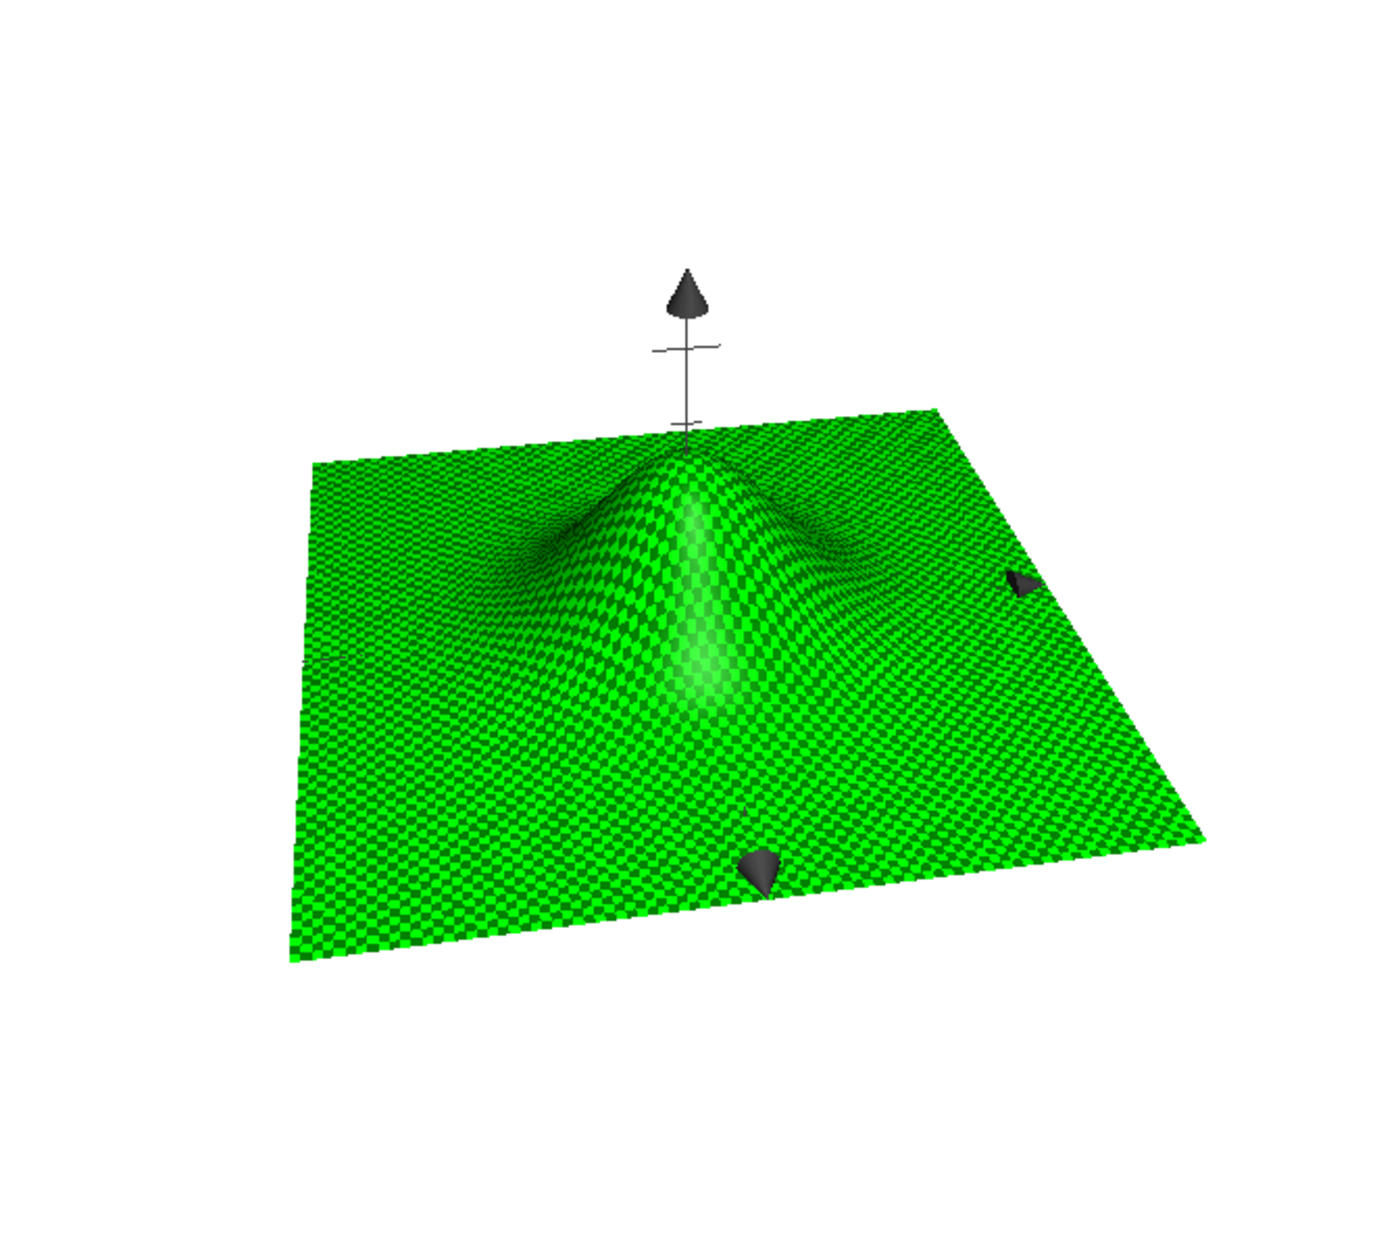
\includegraphics[width=0.4\textwidth]{Uebung6/Gauss.pdf} 
   \caption{$Gauss_{\sigma}(x,y)$}
   \label{fig:Gauss}
\end{figure}

\begin{figure}[p] %  figure placement: here, top, bottom, or page
   \centering
   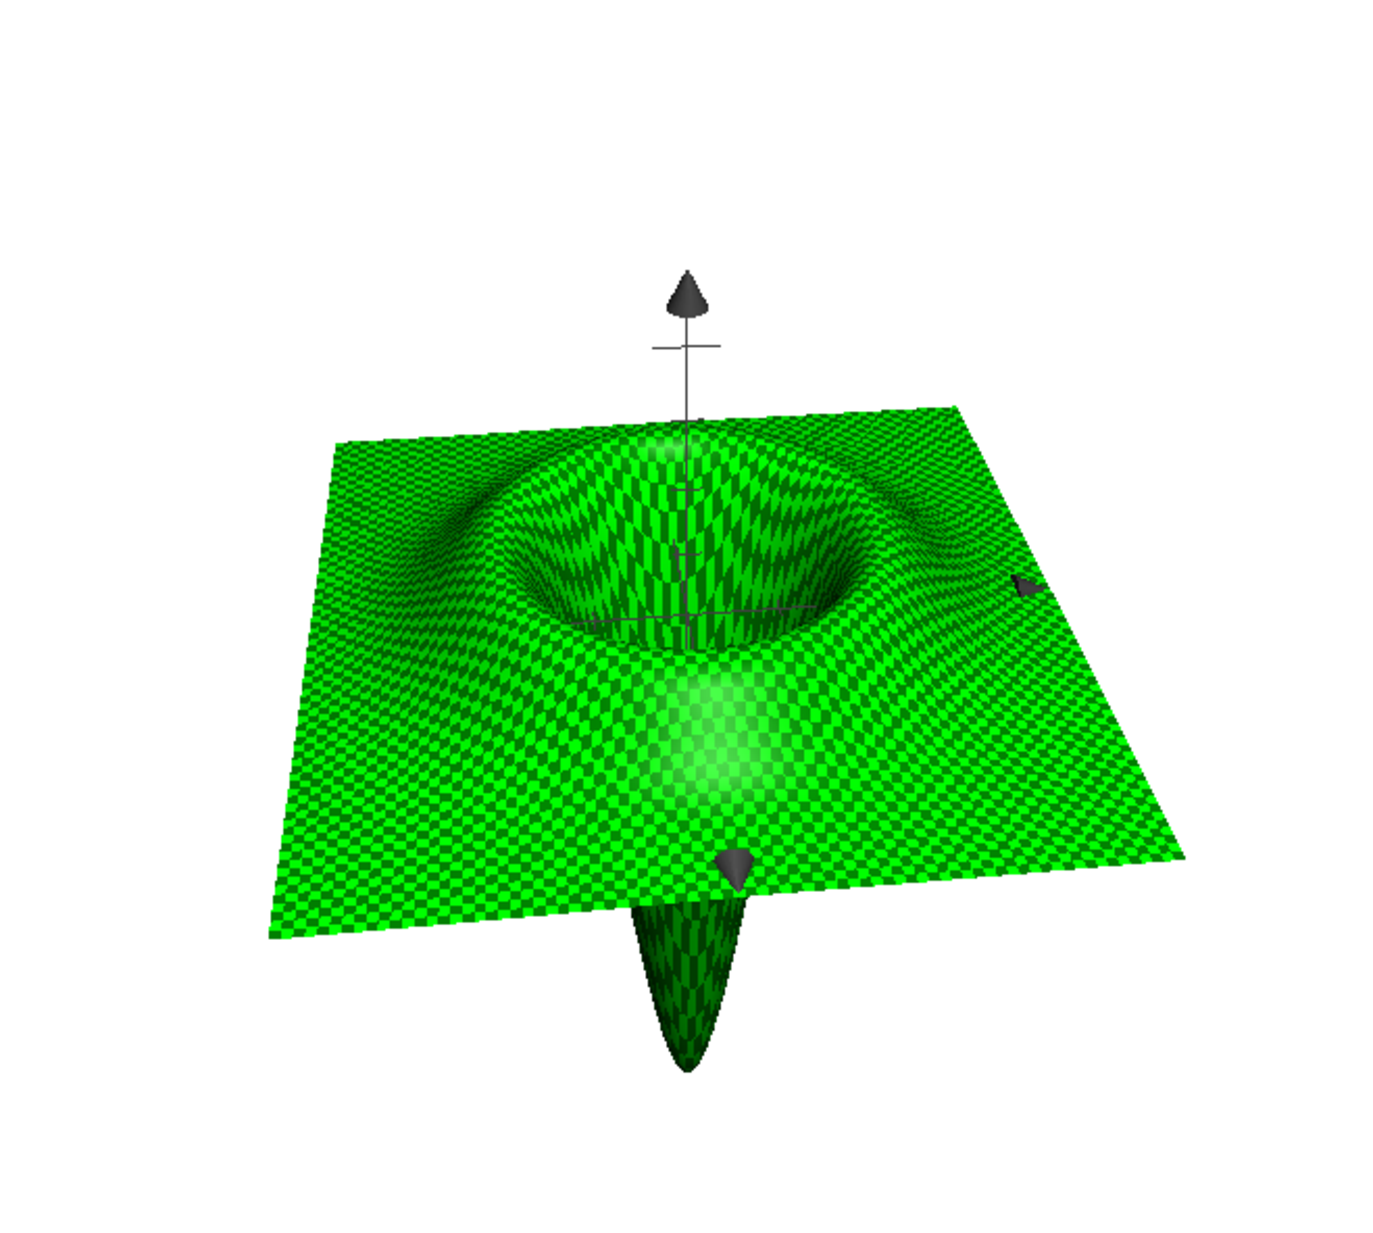
\includegraphics[width=0.4\textwidth]{Uebung6/1Abl_sigma.pdf} 
   \caption{$d^{2}/d\sigma,\sigma=0,5$}
   \label{fig:1Abl}
\end{figure}

\begin{figure}[p] %  figure placement: here, top, bottom, or page
   \centering
   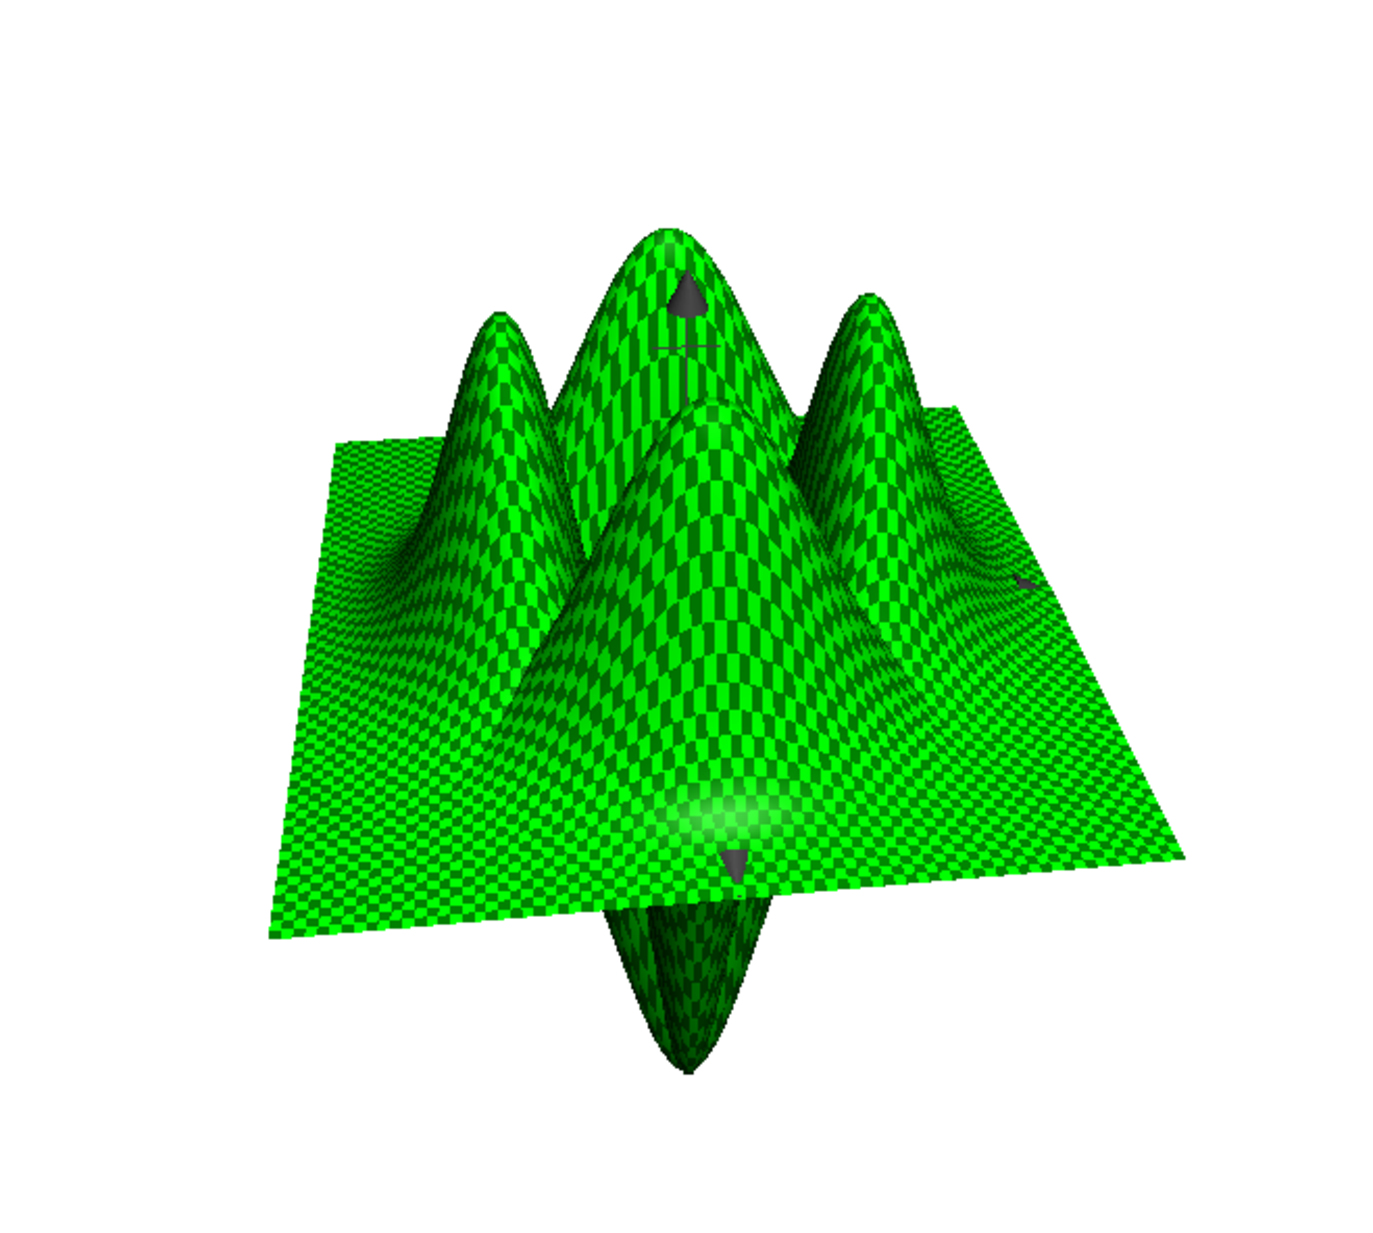
\includegraphics[width=0.4\textwidth]{Uebung6/2Abl_xy.pdf} 
   \caption{$d^{2}/dx^{2}$ und $d^{2}/dy^{2},\sigma=0,5$}
   \label{fig:2Abl}
\end{figure}

\begin{figure}[p] %  figure placement: here, top, bottom, or page
   \centering
   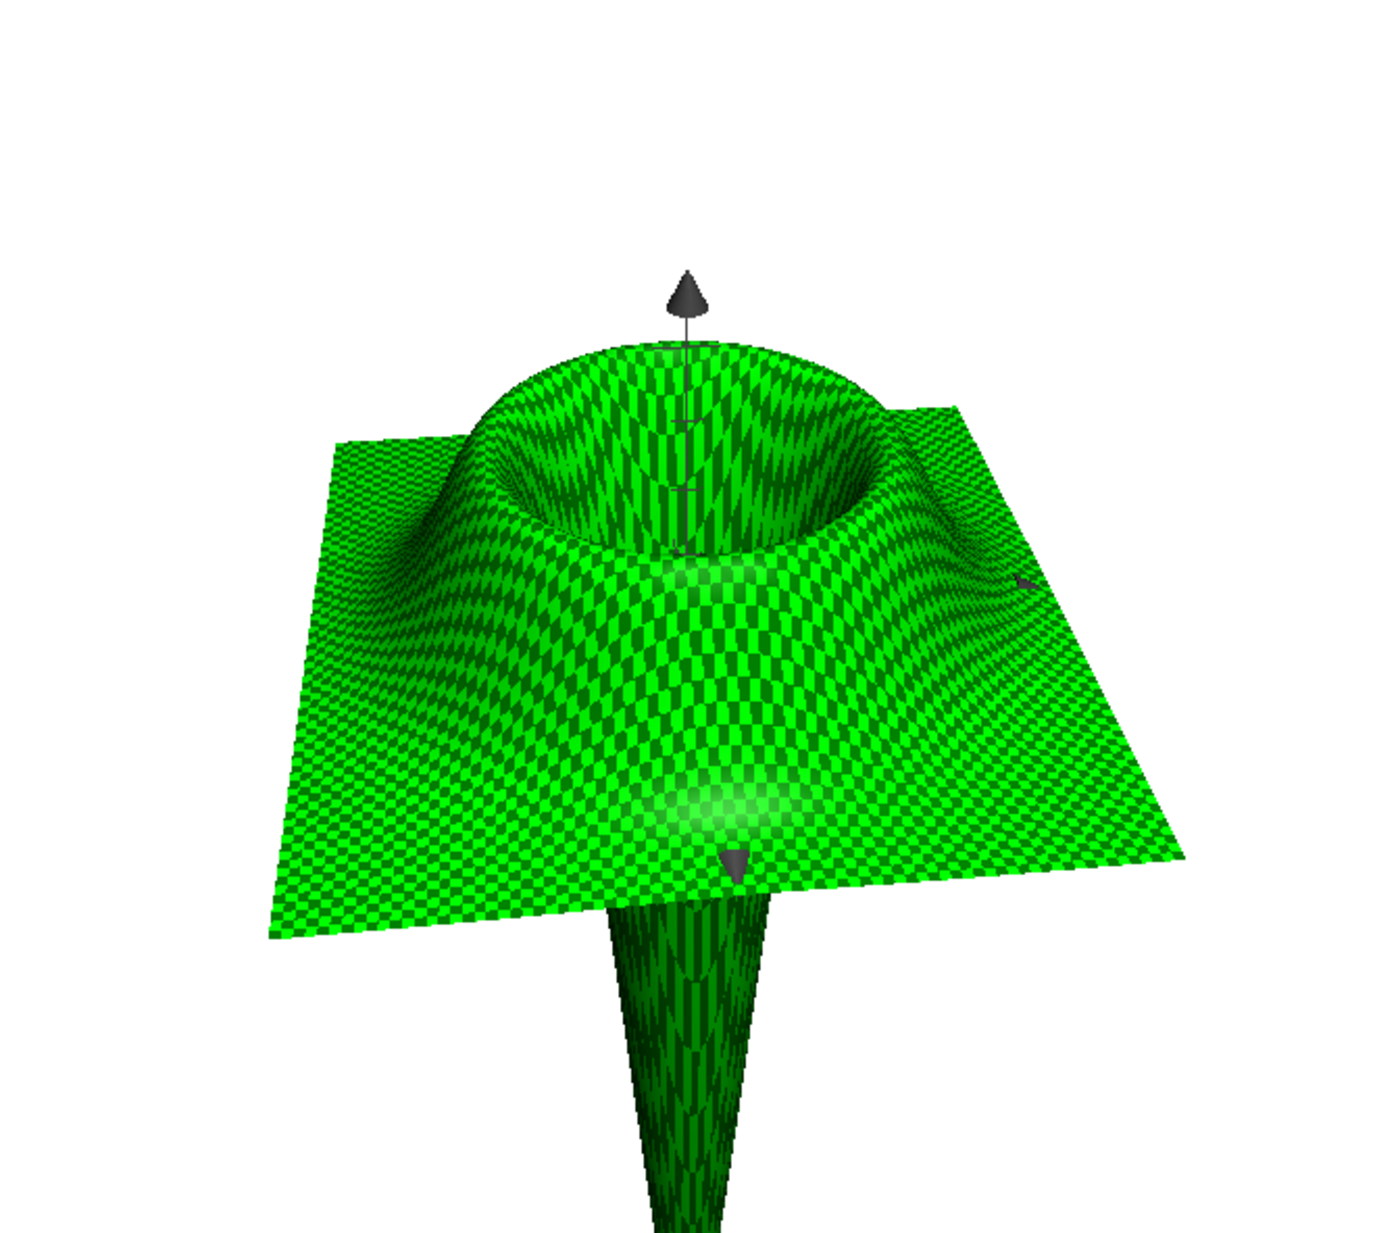
\includegraphics[width=0.4\textwidth]{Uebung6/LoG.pdf} 
   \caption{LoG,$\sigma=0,5$}
   \label{fig:LoG}
\end{figure}

\subsubsection*{Wie kann man den \emph{Laplacian of Gaussion} in einem Gaussian Skalenraum effizient approximieren?}

Den LoG-Operator kann man in diskreten R\"aumen (z.B. dig. Bilder) mit Hilfe einer Matrix (diskreter Kern) approximieren. Dabei entsprechen die Matrix-Elemente dem Funktionswert (neg. und pos.) des LoG-Operators.